% ============================================================
% LLM-BLM 実験 R1：新しい 1,000 社で S1〜S4 を再現し、BLM が比べる相手を上回るかを検定する（事前登録した検定の結果）
% コンパイル：tectonic -X compile LLM-BLM_実験R1.tex   （XeTeX 系。このフォルダで実行する）
% 数値と表は 図/values.tex・図/tab_*.tex（作成スクリプト/values.py）、図は 図/*.pdf（作成スクリプト/figs.py）。
% ============================================================
\documentclass[xelatex,ja=standard,jafont=haranoaji,a4paper,10pt,openany]{bxjsreport}
\setpagelayout*{left=22mm,right=22mm,top=24mm,bottom=26mm,footskip=11mm}

\usepackage{amsmath,amssymb,mathtools,bm}
\usepackage{booktabs,array,multirow,longtable}
\usepackage{graphicx}
\usepackage{adjustbox}
\usepackage{xcolor}
\usepackage{enumitem}
\usepackage{caption}
\usepackage{float}
\usepackage[most]{tcolorbox}
\usepackage[hidelinks,bookmarksnumbered]{hyperref}

\graphicspath{{図/}}
% values.py が results から作る。手で直さない。
\expandafter\def\csname v@commit\endcsname{4a18414}
\expandafter\def\csname v@npanel\endcsname{38,601}
\expandafter\def\csname v@neval\endcsname{16,164}
\expandafter\def\csname v@nevalgpt\endcsname{7,418}
\expandafter\def\csname v@npanelorig\endcsname{38,054}
\expandafter\def\csname v@nevalorig\endcsname{15,997}
\expandafter\def\csname v@RSone\endcsname{再現した}
\expandafter\def\csname v@RStwo\endcsname{再現した}
\expandafter\def\csname v@RSthree\endcsname{再現した}
\expandafter\def\csname v@RSfour\endcsname{再現しなかった}
\expandafter\def\csname v@nreplicated\endcsname{3}
\expandafter\def\csname v@Bex\endcsname{$+$5.3\%}
\expandafter\def\csname v@Bte\endcsname{10.0\%}
\expandafter\def\csname v@Bir\endcsname{$+$0.53}
\expandafter\def\csname v@Blo\endcsname{$+$1.1\%}
\expandafter\def\csname v@Bhi\endcsname{$+$12.2\%}
\expandafter\def\csname v@Bp\endcsname{$<$0.001}
\expandafter\def\csname v@Bdays\endcsname{2,449}
\expandafter\def\csname v@Bverdict\endcsname{支持}
\expandafter\def\csname v@Oex\endcsname{$+$3.0\%}
\expandafter\def\csname v@Oir\endcsname{$+$0.96}
\expandafter\def\csname v@Op\endcsname{0.002}
\expandafter\def\csname v@oSonec\endcsname{$+$76.1}
\expandafter\def\csname v@oSonet\endcsname{$+$3.20}
\expandafter\def\csname v@oSoneperm\endcsname{0.0010}
\expandafter\def\csname v@oStwoc\endcsname{$+$1.51}
\expandafter\def\csname v@oStwot\endcsname{$+$4.01}
\expandafter\def\csname v@oStwoperm\endcsname{0.0010}
\expandafter\def\csname v@oSthreeb\endcsname{1.220}
\expandafter\def\csname v@oSthreec\endcsname{1.219}
\expandafter\def\csname v@oSthreep\endcsname{0.201}
\expandafter\def\csname v@oSfourb\endcsname{1.22}
\expandafter\def\csname v@oSfourc\endcsname{1.05}
\expandafter\def\csname v@oSfourp\endcsname{0.004}
\expandafter\def\csname v@oSfourte\endcsname{3.2\%}
\expandafter\def\csname v@ogptc\endcsname{$+$148.9}
\expandafter\def\csname v@ogptt\endcsname{$+$4.21}
\expandafter\def\csname v@oport\endcsname{$+$0.16\%}
\expandafter\def\csname v@oportt\endcsname{$+$0.73}
\expandafter\def\csname v@ofinal\endcsname{4.899}
\expandafter\def\csname v@oband\endcsname{3.906}
\expandafter\def\csname v@rSonec\endcsname{$+$54.5}
\expandafter\def\csname v@rSonet\endcsname{$+$2.22}
\expandafter\def\csname v@rSoneperm\endcsname{0.0080}
\expandafter\def\csname v@rStwoc\endcsname{$+$1.06}
\expandafter\def\csname v@rStwot\endcsname{$+$3.01}
\expandafter\def\csname v@rStwoperm\endcsname{0.0200}
\expandafter\def\csname v@rSthreeb\endcsname{3.552}
\expandafter\def\csname v@rSthreec\endcsname{3.494}
\expandafter\def\csname v@rSthreep\endcsname{0.287}
\expandafter\def\csname v@rSfourb\endcsname{3.72}
\expandafter\def\csname v@rSfourc\endcsname{3.32}
\expandafter\def\csname v@rSfourp\endcsname{0.148}
\expandafter\def\csname v@rSfourte\endcsname{10.0\%}
\expandafter\def\csname v@rgptc\endcsname{$+$83.9}
\expandafter\def\csname v@rgptt\endcsname{$+$2.53}
\expandafter\def\csname v@rport\endcsname{$-$1.43\%}
\expandafter\def\csname v@rportt\endcsname{$-$0.88}
\expandafter\def\csname v@rfinal\endcsname{6.764}
\expandafter\def\csname v@rband\endcsname{4.882}
\expandafter\def\csname v@onup\endcsname{30}
\expandafter\def\csname v@onupone\endcsname{171}
\expandafter\def\csname v@ondown\endcsname{30}
\expandafter\def\csname v@onstockdays\endcsname{2,953,000}
\expandafter\def\csname v@ogA\endcsname{1.26}
\expandafter\def\csname v@ogwoA\endcsname{1.20}
\expandafter\def\csname v@oshareA\endcsname{9\%}
\expandafter\def\csname v@ogB\endcsname{1.22}
\expandafter\def\csname v@ogwoB\endcsname{1.17}
\expandafter\def\csname v@oshareB\endcsname{9\%}
\expandafter\def\csname v@ogBcal\endcsname{1.05}
\expandafter\def\csname v@ogwoBcal\endcsname{1.01}
\expandafter\def\csname v@oshareBcal\endcsname{9\%}
\expandafter\def\csname v@otopday\endcsname{2020-03-17}
\expandafter\def\csname v@otopactive\endcsname{$-$2\%}
\expandafter\def\csname v@ononeAg\endcsname{1.26}
\expandafter\def\csname v@ononeAte\endcsname{3.8\%}
\expandafter\def\csname v@ononeAex\endcsname{$+$3.5\%}
\expandafter\def\csname v@ononeAir\endcsname{$+$0.93}
\expandafter\def\csname v@ononeAp\endcsname{0.003}
\expandafter\def\csname v@ononeAfinal\endcsname{5.08}
\expandafter\def\csname v@ononeAlo\endcsname{$+$1.2\%}
\expandafter\def\csname v@ononeAhi\endcsname{$+$5.8\%}
\expandafter\def\csname v@ononeAcalg\endcsname{1.04}
\expandafter\def\csname v@ononeAcalte\endcsname{3.1\%}
\expandafter\def\csname v@ononeAcalex\endcsname{$+$2.8\%}
\expandafter\def\csname v@ononeAcalir\endcsname{$+$0.90}
\expandafter\def\csname v@ononeAcalp\endcsname{0.002}
\expandafter\def\csname v@ononeAcalfinal\endcsname{4.82}
\expandafter\def\csname v@ononeAcallo\endcsname{$+$0.9\%}
\expandafter\def\csname v@ononeAcalhi\endcsname{$+$4.8\%}
\expandafter\def\csname v@ononeBg\endcsname{1.22}
\expandafter\def\csname v@ononeBte\endcsname{3.7\%}
\expandafter\def\csname v@ononeBex\endcsname{$+$3.7\%}
\expandafter\def\csname v@ononeBir\endcsname{$+$1.01}
\expandafter\def\csname v@ononeBp\endcsname{$<$0.001}
\expandafter\def\csname v@ononeBfinal\endcsname{5.17}
\expandafter\def\csname v@ononeBlo\endcsname{$+$1.6\%}
\expandafter\def\csname v@ononeBhi\endcsname{$+$5.9\%}
\expandafter\def\csname v@ononeBcalg\endcsname{1.05}
\expandafter\def\csname v@ononeBcalte\endcsname{3.2\%}
\expandafter\def\csname v@ononeBcalex\endcsname{$+$3.0\%}
\expandafter\def\csname v@ononeBcalir\endcsname{$+$0.96}
\expandafter\def\csname v@ononeBcalp\endcsname{0.002}
\expandafter\def\csname v@ononeBcalfinal\endcsname{4.90}
\expandafter\def\csname v@ononeBcallo\endcsname{$+$1.2\%}
\expandafter\def\csname v@ononeBcalhi\endcsname{$+$5.0\%}
\expandafter\def\csname v@ononeband\endcsname{3.91}
\expandafter\def\csname v@omainAg\endcsname{1.27}
\expandafter\def\csname v@omainAte\endcsname{3.8\%}
\expandafter\def\csname v@omainAex\endcsname{$+$3.8\%}
\expandafter\def\csname v@omainAir\endcsname{$+$0.99}
\expandafter\def\csname v@omainAp\endcsname{$<$0.001}
\expandafter\def\csname v@omainAfinal\endcsname{5.17}
\expandafter\def\csname v@omainAlo\endcsname{$+$1.5\%}
\expandafter\def\csname v@omainAhi\endcsname{$+$6.1\%}
\expandafter\def\csname v@omainAcalg\endcsname{1.05}
\expandafter\def\csname v@omainAcalte\endcsname{3.1\%}
\expandafter\def\csname v@omainAcalex\endcsname{$+$2.9\%}
\expandafter\def\csname v@omainAcalir\endcsname{$+$0.93}
\expandafter\def\csname v@omainAcalp\endcsname{0.002}
\expandafter\def\csname v@omainAcalfinal\endcsname{4.84}
\expandafter\def\csname v@omainAcallo\endcsname{$+$1.0\%}
\expandafter\def\csname v@omainAcalhi\endcsname{$+$4.8\%}
\expandafter\def\csname v@omainBg\endcsname{1.26}
\expandafter\def\csname v@omainBte\endcsname{3.8\%}
\expandafter\def\csname v@omainBex\endcsname{$+$3.9\%}
\expandafter\def\csname v@omainBir\endcsname{$+$1.04}
\expandafter\def\csname v@omainBp\endcsname{$<$0.001}
\expandafter\def\csname v@omainBfinal\endcsname{5.23}
\expandafter\def\csname v@omainBlo\endcsname{$+$1.7\%}
\expandafter\def\csname v@omainBhi\endcsname{$+$6.1\%}
\expandafter\def\csname v@omainBcalg\endcsname{1.04}
\expandafter\def\csname v@omainBcalte\endcsname{3.1\%}
\expandafter\def\csname v@omainBcalex\endcsname{$+$3.0\%}
\expandafter\def\csname v@omainBcalir\endcsname{$+$0.97}
\expandafter\def\csname v@omainBcalp\endcsname{$<$0.001}
\expandafter\def\csname v@omainBcalfinal\endcsname{4.88}
\expandafter\def\csname v@omainBcallo\endcsname{$+$1.2\%}
\expandafter\def\csname v@omainBcalhi\endcsname{$+$4.9\%}
\expandafter\def\csname v@omainband\endcsname{3.89}
\expandafter\def\csname v@onremoved\endcsname{60}
\expandafter\def\csname v@oreproduces\endcsname{一致した}
\expandafter\def\csname v@rnup\endcsname{38}
\expandafter\def\csname v@rnupone\endcsname{203}
\expandafter\def\csname v@rndown\endcsname{31}
\expandafter\def\csname v@rnstockdays\endcsname{2,953,000}
\expandafter\def\csname v@rgA\endcsname{2.22}
\expandafter\def\csname v@rgwoA\endcsname{1.14}
\expandafter\def\csname v@rshareA\endcsname{74\%}
\expandafter\def\csname v@rgB\endcsname{3.72}
\expandafter\def\csname v@rgwoB\endcsname{1.11}
\expandafter\def\csname v@rshareB\endcsname{91\%}
\expandafter\def\csname v@rgBcal\endcsname{3.32}
\expandafter\def\csname v@rgwoBcal\endcsname{0.89}
\expandafter\def\csname v@rshareBcal\endcsname{93\%}
\expandafter\def\csname v@rtopday\endcsname{2020-11-20}
\expandafter\def\csname v@rtopactive\endcsname{$+$30\%}
\expandafter\def\csname v@rnoneAg\endcsname{2.22}
\expandafter\def\csname v@rnoneAte\endcsname{6.6\%}
\expandafter\def\csname v@rnoneAex\endcsname{$+$5.0\%}
\expandafter\def\csname v@rnoneAir\endcsname{$+$0.75}
\expandafter\def\csname v@rnoneAp\endcsname{$<$0.001}
\expandafter\def\csname v@rnoneAfinal\endcsname{6.80}
\expandafter\def\csname v@rnoneAlo\endcsname{$+$1.8\%}
\expandafter\def\csname v@rnoneAhi\endcsname{$+$9.3\%}
\expandafter\def\csname v@rnoneAcalg\endcsname{1.91}
\expandafter\def\csname v@rnoneAcalte\endcsname{5.7\%}
\expandafter\def\csname v@rnoneAcalex\endcsname{$+$3.9\%}
\expandafter\def\csname v@rnoneAcalir\endcsname{$+$0.68}
\expandafter\def\csname v@rnoneAcalp\endcsname{$<$0.001}
\expandafter\def\csname v@rnoneAcalfinal\endcsname{6.23}
\expandafter\def\csname v@rnoneAcallo\endcsname{$+$1.3\%}
\expandafter\def\csname v@rnoneAcalhi\endcsname{$+$7.6\%}
\expandafter\def\csname v@rnoneBg\endcsname{3.72}
\expandafter\def\csname v@rnoneBte\endcsname{11.1\%}
\expandafter\def\csname v@rnoneBex\endcsname{$+$6.5\%}
\expandafter\def\csname v@rnoneBir\endcsname{$+$0.59}
\expandafter\def\csname v@rnoneBp\endcsname{$<$0.001}
\expandafter\def\csname v@rnoneBfinal\endcsname{7.44}
\expandafter\def\csname v@rnoneBlo\endcsname{$+$1.7\%}
\expandafter\def\csname v@rnoneBhi\endcsname{$+$14.2\%}
\expandafter\def\csname v@rnoneBcalg\endcsname{3.32}
\expandafter\def\csname v@rnoneBcalte\endcsname{10.0\%}
\expandafter\def\csname v@rnoneBcalex\endcsname{$+$5.3\%}
\expandafter\def\csname v@rnoneBcalir\endcsname{$+$0.53}
\expandafter\def\csname v@rnoneBcalp\endcsname{$<$0.001}
\expandafter\def\csname v@rnoneBcalfinal\endcsname{6.76}
\expandafter\def\csname v@rnoneBcallo\endcsname{$+$1.1\%}
\expandafter\def\csname v@rnoneBcalhi\endcsname{$+$12.2\%}
\expandafter\def\csname v@rnoneband\endcsname{4.88}
\expandafter\def\csname v@rmainAg\endcsname{1.26}
\expandafter\def\csname v@rmainAte\endcsname{3.8\%}
\expandafter\def\csname v@rmainAex\endcsname{$+$3.0\%}
\expandafter\def\csname v@rmainAir\endcsname{$+$0.79}
\expandafter\def\csname v@rmainAp\endcsname{0.003}
\expandafter\def\csname v@rmainAfinal\endcsname{4.19}
\expandafter\def\csname v@rmainAlo\endcsname{$+$0.8\%}
\expandafter\def\csname v@rmainAhi\endcsname{$+$5.2\%}
\expandafter\def\csname v@rmainAcalg\endcsname{1.08}
\expandafter\def\csname v@rmainAcalte\endcsname{3.2\%}
\expandafter\def\csname v@rmainAcalex\endcsname{$+$2.8\%}
\expandafter\def\csname v@rmainAcalir\endcsname{$+$0.86}
\expandafter\def\csname v@rmainAcalp\endcsname{0.001}
\expandafter\def\csname v@rmainAcalfinal\endcsname{4.16}
\expandafter\def\csname v@rmainAcallo\endcsname{$+$0.9\%}
\expandafter\def\csname v@rmainAcalhi\endcsname{$+$4.7\%}
\expandafter\def\csname v@rmainBg\endcsname{1.24}
\expandafter\def\csname v@rmainBte\endcsname{3.7\%}
\expandafter\def\csname v@rmainBex\endcsname{$+$3.1\%}
\expandafter\def\csname v@rmainBir\endcsname{$+$0.84}
\expandafter\def\csname v@rmainBp\endcsname{0.003}
\expandafter\def\csname v@rmainBfinal\endcsname{4.25}
\expandafter\def\csname v@rmainBlo\endcsname{$+$0.9\%}
\expandafter\def\csname v@rmainBhi\endcsname{$+$5.3\%}
\expandafter\def\csname v@rmainBcalg\endcsname{1.08}
\expandafter\def\csname v@rmainBcalte\endcsname{3.2\%}
\expandafter\def\csname v@rmainBcalex\endcsname{$+$2.9\%}
\expandafter\def\csname v@rmainBcalir\endcsname{$+$0.89}
\expandafter\def\csname v@rmainBcalp\endcsname{$<$0.001}
\expandafter\def\csname v@rmainBcalfinal\endcsname{4.19}
\expandafter\def\csname v@rmainBcallo\endcsname{$+$1.0\%}
\expandafter\def\csname v@rmainBcalhi\endcsname{$+$4.8\%}
\expandafter\def\csname v@rmainband\endcsname{3.52}
\expandafter\def\csname v@rnremoved\endcsname{69}
\expandafter\def\csname v@rreproduces\endcsname{一致した}
\expandafter\def\csname v@obigjumps\endcsname{AMPY（2016-10-24、$+$16,079\%）、NFE（2026-08-04、$+$5,064\%）、NFE（2026-08-07、$+$5,060\%）}
\expandafter\def\csname v@rbigjumps\endcsname{CHRD（2020-11-20、$+$25,733\%）、DFTX（2019-12-27、$+$4,700\%）、TPST（2023-10-11、$+$3,971\%）}

\newcommand{\V}[1]{\ifcsname v@#1\endcsname\csname v@#1\endcsname\else\textbf{??#1??}\fi}
\newcommand{\tabin}[1]{\adjustbox{max width=\linewidth}{\input{図/tab_#1.tex}}}

\definecolor{c1}{HTML}{2A78D6}
\definecolor{soft1}{HTML}{E4EEF9}

\newcommand{\code}[1]{\texttt{#1}}
\newcommand{\SP}{S\&P500}
\newcommand{\figref}[1]{図~\ref{#1}}
\newcommand{\tabref}[1]{表~\ref{#1}}
\newcommand{\chapref}[1]{第~\ref{#1}~章}

\setlist[itemize]{leftmargin=1.6em,itemsep=0.2em,topsep=0.4em}
\setlist[enumerate]{leftmargin=1.8em,itemsep=0.2em,topsep=0.4em}
\captionsetup{font=small,labelfont=bf,skip=6pt}
\renewcommand{\arraystretch}{1.2}

\makeatletter
\def\@makechapterhead#1{\vspace*{0.3\Cvs}{\parindent\z@\raggedright\normalfont
  \ifnum\c@secnumdepth>\m@ne\if@mainmatter{\Large\headfont\@chapapp\thechapter\@chappos}\par\nobreak\vskip0.4\Cvs\fi\fi
  \interlinepenalty\@M\LARGE\headfont #1\par\nobreak\vskip 1.5\Cvs}}
\def\@makeschapterhead#1{\vspace*{0.3\Cvs}{\parindent\z@\raggedright\normalfont
  \interlinepenalty\@M\LARGE\headfont #1\par\nobreak\vskip 1.5\Cvs}}
\makeatother

\newtcolorbox{keybox}[1][要点]{enhanced,breakable,colback=soft1,colframe=c1,boxrule=0.5pt,arc=2pt,
  left=8pt,right=8pt,top=6pt,bottom=6pt,title={#1},fonttitle=\sffamily\bfseries\small,coltitle=white}

\title{LLM-BLM 実験 R1\\[6pt]
  \large 新しい 1,000 社での S1〜S4 の再現と、\\BLM が比べる相手を上回るかの検定}
\author{実験の報告書（事前登録した検定の結果）}
\date{2026 年 10 月 25 日}

\begin{document}
\maketitle

\chapter*{概要}
\addcontentsline{toc}{chapter}{概要}

小型株の実験 S1〜S4 は、同じ 1,000 社（元の標本）で行った。この実験 R1 では、元の標本に含まれない新しい 1,000 社で S1〜S4 を同じコード・同じ設定で 1 回ずつやり直し（再現）、あわせて、S4 の形の BLM が比べる相手（範囲の全社、浮動株時価総額で加重）を上回るかを、新しい主な検定（R-BLM）として事前登録して確かめた。

\begin{keybox}[要点]
\begin{itemize}
\item \textbf{4 つの主な検定のうち \V{nreplicated} つが再現した}。決算発表文の読み取りが発表後 2〜60 日のドリフトを予測すること（S1：\V{rSonec}bp/SD、$t$ = \V{rSonet}、並べ替えの $p$ = \V{rSoneperm}）、発表後の変動率を予測すること（S2：\V{rStwoc}\%/SD、$t$ = \V{rStwot}）、文章のリスクの点数で共分散を補正しても TE の見積もりは良くならないこと（S3）は、新しい標本でも同じだった。TE の校正（S4）は再現しなかった。
\item \textbf{R-BLM は、事前登録の基準では\V{Bverdict}された}（2017 年以降、比べる相手との差は年 \V{Bex}、95\% 区間 [\V{Blo}, \V{Bhi}]、片側 $p$ \V{Bp}）。ただし実現の TE は \V{Bte} で、約束の 3\% の約 3 倍だった。
\item \textbf{探索（結果を見た後の分析）で、その原因は株価データの誤りだとわかった}。\V{rtopday} に、破産から再出発した会社（CHRD）の古い株と新しい株の価格を yfinance がつないでいて、1 日で約 +25{,}700\% の、実際にはなかった値上がりが入っていた。この 1 日だけで、BLM と相手の差が \V{rtopactive} 開き、そのあと約 3 年、校正が TE の上限を下限の 1\% に張り付かせた。
\item \textbf{ありえない日々のリターン（+300\% 超、$-$80\% 未満）を除いて計算し直すと}、新しい標本でも校正は元の標本と同じように効いた（偏り $g$：校正なし \V{rmainBg} → 校正あり \V{rmainBcalg}。元の標本は \V{omainBg} → \V{omainBcalg}）。S4 の不成立は、この種のデータの誤りでほぼ説明できる。
\item 誤りを除いた後の R-BLM の BLM は、新しい標本で実現の TE \V{rmainBcalte}、相手との差は年 \V{rmainBcalex}（95\% 区間 [\V{rmainBcallo}, \V{rmainBcalhi}]、片側 $p$ \V{rmainBcalp}）、元の標本で差は年 \V{omainBcalex}（片側 $p$ \V{omainBcalp}）だった。事前登録の値（年 \V{Bex}）の多くは誤りから来ていたが、誤りを除いても、両方の標本で相手を上回った。これは結果を見た後の分析なので、誤りを除く規則を先に決めて、別の期間で確かめ直す必要がある。
\item 同じ種類のデータの誤りは元の標本にもあった。これからの小型株の計算では、株価の誤りを先に取り除く手順を、事前登録に入れる。
\end{itemize}
\end{keybox}


\setcounter{tocdepth}{1}
{\small\tableofcontents}

% ============================================================
\chapter{目的}\label{ch:purpose}

S1〜S4 は、同じ 1,000 社（元の標本）で行った。S1 の検定自体は事前登録して 1 回だけ実行したが、S2〜S4 の設計は S1 の結果を見た後であり、BLM の推移が比べる相手を上回ったことは検定していなかった。そこで、次の 2 つを、元の標本に含まれない新しい 1,000 社で確かめた。

\begin{keybox}[問い]
\begin{enumerate}
\item S1〜S4 の主な検定の結果は、別の 1,000 社でも同じになるか（再現）。
\item S4 の形の BLM（ChronoGPT の見通し・株価で補正した共分散・TE の校正）は、比べる相手（範囲の全社、浮動株時価総額で加重）を上回るか（新しい主な検定）。
\end{enumerate}
\end{keybox}

% ============================================================
\chapter{事前登録と方法}\label{ch:method}

仮説・方法・判定の基準は \code{experiments/R1\_replication/preregistration.md} に書き、コードと同じコミットで固定してから実行した。新しい標本の株価の反応・変動率・ポートフォリオは、それまで一度も計算していない。

\section{新しい標本}

元の標本を選んだのと同じ条件（小型株の範囲に一度でも入った会社のうち、いま上場して株価があり、2016 年以降の決算の 8-K が 4 件以上）を満たす 2,400 社から、元の 1,000 社を除いた 1,400 社のうち、1,000 社を乱数の種 1 で選んだ（元の標本との重なりは 0）。決算発表文・財務データ・驚き・点数（辞書、FinBERT、ChronoGPT、gpt-4o-mini）は、元の標本と同じコードで作った。

2015 年以降の発表は \V{npanel} 件（元の標本は \V{npanelorig} 件）、評価する発表（2020 年以降、範囲の中）は \V{neval} 件（元は \V{nevalorig} 件）。

\section{実行}

S1〜S4 のコードを、データベース・点数の保存先・結果のフォルダだけを環境変数で切り替えて、元と同じ順・同じ設定・同じ乱数の種で 1 回ずつ実行した。

\section{再現の判定}

S1・S2・S4 の主な検定は、元と同じ基準で「支持」なら「再現した」。S3 の主な検定は、元の結果が「支持されない」だったので、再び「支持されない」なら「再現した（効果なし）」とした。

\section{新しい主な検定（R-BLM）}

2015 年末から四半期ごと、ChronoGPT＋リッジの見通し、株価で補正した共分散（B）、TE の校正ありの BLM について、2017 年以降の日次の超過リターン（BLM − 比べる相手）の平均が正かを、円形のブロック・ブートストラップ（ブロック 63 日、2,000 回）で検定した（片側 $p < 0.05$ で「支持」）。

% ============================================================
% 結果の章（数値は 図/values.tex と 図/tab_*.tex から。手で書かない）

% ============================================================
\chapter{再現の判定}\label{ch:replication}

\begin{table}[H]
\centering\small
\caption{S1〜S4 の主な検定：元の標本と新しい標本}
\label{tab:replication}
\begin{adjustbox}{max width=\linewidth}
\begin{tabular}{@{}llrrl@{}}
\toprule
実験 & 主な数字 & 元の標本 & 新しい標本 & 判定 \\
\midrule
S1：ドリフトの予測（ChronoGPT＋リッジ → 2〜60 日の超過リターン） & 係数（bp/SD） & \V{oSonec} & \V{rSonec} & \textbf{\V{RSone}} \\
 & $t$ & \V{oSonet} & \V{rSonet} & \\
 & 並べ替えの片側 $p$ & \V{oSoneperm} & \V{rSoneperm} & \\
S2：変動率の予測（ChronoGPT＋リッジ → 2〜60 日の変動率） & 係数（\%/SD） & \V{oStwoc} & \V{rStwoc} & \textbf{\V{RStwo}} \\
 & $t$ & \V{oStwot} & \V{rStwot} & \\
 & 並べ替えの片側 $p$ & \V{oStwoperm} & \V{rStwoperm} & \\
S3：文章のリスクの点数で共分散を補正（B → C） & 偏り $b$（B） & \V{oSthreeb} & \V{rSthreeb} & \textbf{\V{RSthree}}（効果なし） \\
 & 偏り $b$（C） & \V{oSthreec} & \V{rSthreec} & \\
 & 片側 $p$ & \V{oSthreep} & \V{rSthreep} & \\
S4：TE の上限の校正（B → B＋校正） & $g$（B） & \V{oSfourb} & \V{rSfourb} & \textbf{\V{RSfour}} \\
 & $g$（B＋校正） & \V{oSfourc} & \V{rSfourc} & \\
 & 実現の TE（B＋校正） & \V{oSfourte} & \V{rSfourte} & \\
 & 片側 $p$ & \V{oSfourp} & \V{rSfourp} & \\
\bottomrule
\end{tabular}
\end{adjustbox}
\end{table}

評価した発表は、新しい標本で \V{neval} 件（元の標本は \V{nevalorig} 件）、gpt-4o-mini の期間（2024 年以降）は \V{nevalgpt} 件。偏り $b$ = 日々の（BLM − 相手）÷ 事前の TE の 2 乗平均の平方根、$g$ = 日々の（BLM − 相手）÷（3\%$/\sqrt{252}$）の 2 乗平均の平方根（どちらも 1 なら見積もりどおり）。

\begin{keybox}[結果]
\textbf{4 つのうち \V{nreplicated} つが再現した}。
\begin{itemize}
\item \textbf{S1（ドリフト）}：係数は元の \V{oSonec}bp から \V{rSonec}bp に小さくなったが、$t$ = \V{rSonet}、並べ替えの $p$ = \V{rSoneperm} で、同じ基準を満たした。
\item \textbf{S2（変動率）}：\V{rStwoc}\%/SD（$t$ = \V{rStwot}）。元より小さいが、同じ向きではっきりしている。
\item \textbf{S3（文章による共分散の補正）}：元と同じく、補正しても偏りは変わらなかった（効果がないことが再現した）。
\item \textbf{S4（TE の校正）}：再現しなかった。新しい標本では偏りが \V{rSfourb} と大きく（元は \V{oSfourb}）、校正しても \V{rSfourc}（実現の TE \V{rSfourte}）にしか下がらなかった。原因は \chapref{ch:explore} の探索で調べた。
\end{itemize}
\end{keybox}

\begin{figure}[H]
\centering
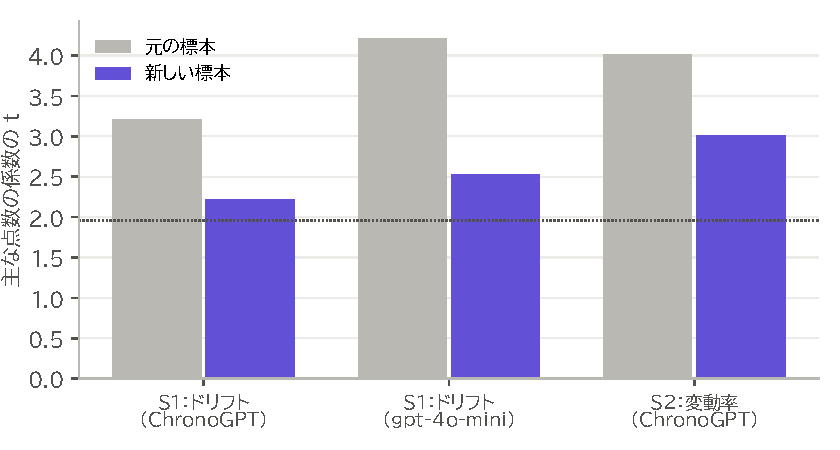
\includegraphics[width=0.72\linewidth]{coef.pdf}
\caption{主な点数の係数の $t$。点線は 1.96。S1 の gpt-4o-mini は副次の検定（2024 年以降）。}
\label{fig:coef}
\end{figure}

gpt-4o-mini の読み取り（学習なし）も、新しい標本でドリフトを予測した（\V{rgptc}bp/SD、$t$ = \V{rgptt}。元は \V{ogptc}bp、$t$ = \V{ogptt}）。

S1 の副次の月次のポートフォリオ（点数の上位 5 分の 1 を浮動株時価総額で持つ、片道 0.3\% の費用の後）は、元の標本で月 \V{oport}（$t$ = \V{oportt}）、新しい標本で月 \V{rport}（$t$ = \V{rportt}）で、どちらも比べる相手との差ははっきりしなかった。

% ============================================================
\chapter{新しい主な検定（R-BLM）}\label{ch:rblm}

\begin{keybox}[結果]
事前登録の基準では\textbf{\V{Bverdict}された}。2015 年末から四半期ごとの BLM（ChronoGPT＋リッジ、共分散 B、TE の校正あり）の、2017 年以降 \V{Bdays} 日の比べる相手との差は年 \V{Bex}（95\% 区間 [\V{Blo}, \V{Bhi}]、片側 $p$ \V{Bp}）、情報レシオ \V{Bir}。

\textbf{ただし実現の TE は \V{Bte} で、約束の 3\% の約 3 倍だった}。この差の多くは 1 日のデータの誤りから来ている（\chapref{ch:explore}）。
\end{keybox}

\begin{table}[H]
\centering\small
\caption{BLM と比べる相手の差（年率、評価する日）。主な検定は 1 行目。ほかは副次（判定には使わない）。元の標本の列は、R1 の事前登録を書いた時点で一度計算していた探索の値}
\label{tab:blm}
\tabin{blm}
\end{table}

\begin{figure}[H]
\centering
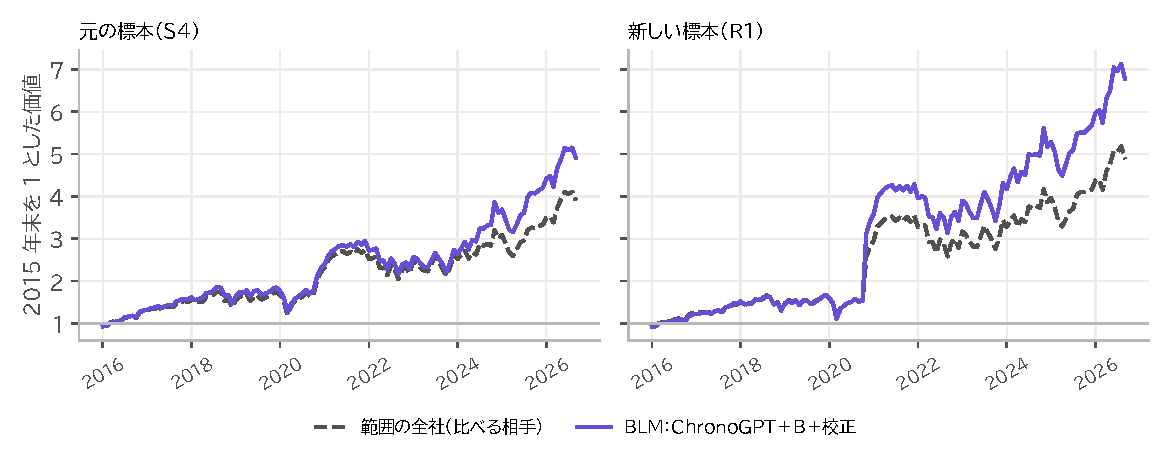
\includegraphics[width=\linewidth]{paths.pdf}
\caption{2015 年末を 1 とした推移（四半期ごと、ChronoGPT＋リッジ、共分散 B、TE の校正あり）。新しい標本の 2020 年 11 月の跳ね上がりの多くは、比べる相手にも BLM にも入っている株価の誤り（\chapref{ch:explore}）。}
\label{fig:paths}
\end{figure}

最終の値は、元の標本で BLM \V{ofinal}・相手 \V{oband}、新しい標本で BLM \V{rfinal}・相手 \V{rband}。

% ============================================================
\chapter{探索：TE が約束の約 3 倍になった理由}\label{ch:explore}

\textbf{この章は事前登録していない}。R1 の結果を見た後に、新しい標本で実現の TE が大きかった理由を調べた（\code{experiments/R1\_replication/explore.py}、結果は \code{results/explore\_orig.json}・\code{explore\_rep.json}）。ここの数字で、前の章の判定は変えない。

\section{1 日の寄与}

\begin{figure}[H]
\centering
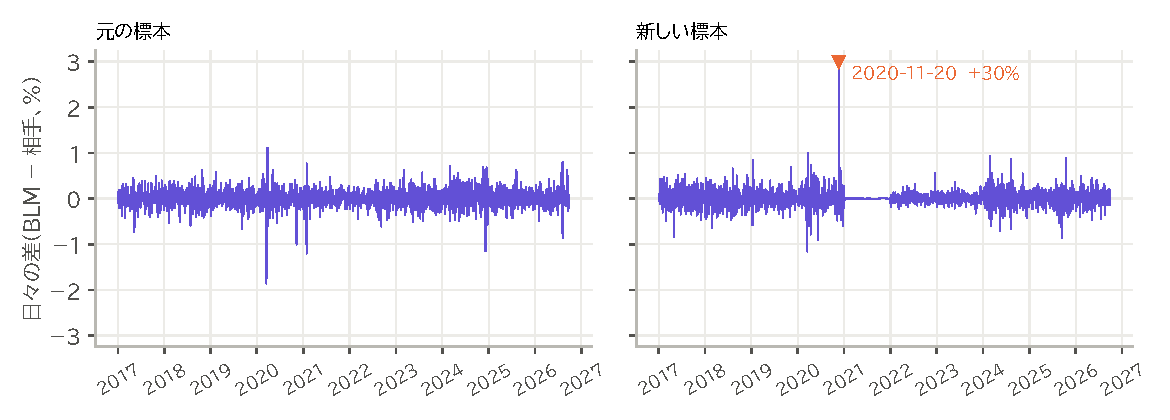
\includegraphics[width=\linewidth]{active.pdf}
\caption{日々の差（BLM − 比べる相手、\%）。2017 年以降、四半期ごと、共分散 B、TE の校正あり。$\pm$3\% を超える日は端に印を付けた。}
\label{fig:active}
\end{figure}

新しい標本では、\V{rtopday} の 1 日に、BLM と相手の差が \V{rtopactive} 開いた。日々の差の 2 乗の合計のうち、いちばん大きい 5 日が占める割合は、新しい標本で \V{rshareBcal}（元の標本は \V{oshareBcal}）。この 5 日を除くと、偏り $g$ は次のようになる。

\begin{table}[H]
\centering\small
\caption{偏り $g$（2017 年以降、四半期ごと）と、いちばん大きい 5 日を除いた値}
\label{tab:top5}
\begin{tabular}{@{}lrrrr@{}}
\toprule
 & \multicolumn{2}{c}{元の標本} & \multicolumn{2}{c}{新しい標本} \\
\cmidrule(lr){2-3}\cmidrule(lr){4-5}
共分散 & $g$ & 5 日を除く & $g$ & 5 日を除く \\
\midrule
A（補正なし） & \V{ogA} & \V{ogwoA} & \V{rgA} & \V{rgwoA} \\
B（株価で補正） & \V{ogB} & \V{ogwoB} & \V{rgB} & \V{rgwoB} \\
B＋校正 & \V{ogBcal} & \V{ogwoBcal} & \V{rgBcal} & \V{rgwoBcal} \\
\bottomrule
\end{tabular}
\end{table}

5 日を除くと、新しい標本の偏りは元の標本と同じくらいになり、校正すると 1 を下回った。

\section{原因：破産から再出発した会社の株価のつなぎ}

その日に大きく動いたのは CHRD（今の Chord Energy。2020 年当時は Oasis Petroleum）だった。Oasis は 2020 年に連邦破産法 11 条の手続きに入り、2020 年 11 月に新しい株で再出発した。古い株は取り消されて新しい株が発行されたので、古い株を持っていた人の資産が 1 日で 250 倍になったわけではない。ところが yfinance は、古い株の最後の価格（0.12 ドル）に新しい株の最初の価格（31 ドル）をそのままつないでいて、調整後終値の日々のリターンは \V{rtopday} に約 +25{,}700\% になっていた。

BLM はこの銘柄を相手より約 0.1\% 多く持っていたので、この 1 日で差が大きく開いた。比べる相手も浮動株時価総額でこの銘柄を持っていたので、相手の価値も同じ日に跳ね上がった（\figref{fig:paths}）。さらに、TE の校正は過去 756 日の偏りで上限を割るので、この 1 日が過去 756 日に入っていた 2020 年 12 月から 2023 年 9 月まで（12 回のリバランス、約 3 年）、上限は下限の 1\% に張り付き、BLM の動きは小さくなった（\figref{fig:active}）。

同じような日は、両方の標本にあった。

\begin{table}[H]
\centering\small
\caption{標本の会社の日々のリターン（調整後終値、2015 年以降）のうち、ありえない大きさのもの}
\label{tab:extreme}
\begin{tabular}{@{}lrr@{}}
\toprule
 & 元の標本 & 新しい標本 \\
\midrule
会社 × 日の数 & \V{onstockdays} & \V{rnstockdays} \\
$+$300\% を超える日 & \V{onup} & \V{rnup} \\
$+$100\% を超える日 & \V{onupone} & \V{rnupone} \\
$-$80\% を下回る日 & \V{ondown} & \V{rndown} \\
\bottomrule
\end{tabular}
\end{table}

いちばん大きいもの：元の標本は \V{obigjumps}、新しい標本は \V{rbigjumps}。破産からの再出発のつなぎのほか、1 日で何十倍にもなって翌日に元へ戻る、価格の乱れもあった。

\section{ありえないリターンを除いた計算}

S4 の 2015 年末から四半期ごとのポートフォリオを、日々のリターンのうちしきい値を超えるものを欠け（S4 は欠けた価格を 0\% と数える）として、計算し直した。しきい値は、計算する前に 3 通り決めた（主：$+$300\% 超か $-$80\% 未満）。そのままの計算は S4 の値と\V{rreproduces}（元の標本でも\V{oreproduces}）。

\begin{table}[H]
\centering\small
\caption{ありえない日々のリターンを除いた計算（2017 年以降、四半期ごと、ChronoGPT＋リッジ）。最終の値は 2015 年末を 1 とした 2026 年 9 月末の値}
\label{tab:explore}
\tabin{explore}
\end{table}

\begin{keybox}[探索の結果]
\begin{itemize}
\item 主のしきい値で除くと（新しい標本で \V{rnremoved} 個の会社 × 日）、新しい標本の B＋校正の偏りは $g$ = \V{rmainBcalg}（実現の TE \V{rmainBcalte}）になり、約束の 3\% に近づいた。比べる相手との差は年 \V{rmainBcalex}（95\% 区間 [\V{rmainBcallo}, \V{rmainBcalhi}]、片側 $p$ \V{rmainBcalp}）、情報レシオ \V{rmainBcalir}。
\item 元の標本では、除いても結果はほとんど変わらなかった（差は年 \V{omainBcalex}、片側 $p$ \V{omainBcalp}、$g$ = \V{omainBcalg}）。
\item \textbf{誤りを除くと、新しい標本でも TE の校正は効いた}。偏り $g$ は、校正なしの B で \V{rmainBg}、B＋校正で \V{rmainBcalg}（元の標本は \V{omainBg} → \V{omainBcalg}）。S4 が再現しなかったのは、主にこの種の誤りのためだった。
\item 比べる相手の最終の値も、新しい標本ではそのままの \V{rnoneband} から \V{rmainband} に下がった。2020 年 11 月の跳ね上がりの多くが誤りだったことを裏づける。
\item つまり、R-BLM の年 \V{Bex} の多くは株価の誤りから来ていた。誤りを除いた後の値が、この BLM の成績の、より正直な見積もりである。ただし、これは結果を見た後の分析なので、別の標本か別の期間で、誤りを除く手順を先に決めて確かめ直す必要がある。
\item ほかの 2 つのしきい値でも、結論は同じ向きだった（\tabref{tab:explore}）。最適化が解けなかったリバランスは、比べる相手の比率のままにした（S4 が解けないときと同じ扱い）。
\end{itemize}
\end{keybox}

% ============================================================
\chapter{まとめ}\label{ch:summary}

\begin{itemize}
\item \textbf{決算発表文の読み取りが、小型株の発表後のドリフトと変動率を予測することは、別の 1,000 社でも再現した}（S1・S2）。係数は元の標本より小さかった。
\item \textbf{文章のリスクの点数で共分散を補正しても、TE の見積もりは良くならない}ことも再現した（S3）。
\item \textbf{TE の校正（S4）と R-BLM は、株価データの誤り 1 日に大きく左右された}。事前登録の判定（S4 は再現しない、R-BLM は支持）はそのまま記録するが、どちらも誤りの影響を受けた結果である。
\item \textbf{誤りを除くと（探索）}、TE の校正は両方の標本で効き（実現の TE 約 3\%）、BLM は両方の標本で比べる相手を年 約 3\% 上回った（新しい標本 \V{rmainBcalex}、元の標本 \V{omainBcalex}）。事前登録の値（年 \V{Bex}）の約半分は誤りによる上乗せだった。
\item \textbf{これからの手順}：小型株の株価は、計算の前に、ありえない日々のリターン（破産からの再出発のつなぎ、1 日だけの乱れ）を取り除く。その規則を事前登録に書いてから、BLM の検定をやり直す。
\end{itemize}


% ============================================================
\chapter{限界}\label{ch:limits}

\begin{itemize}
\item \textbf{株価データの誤り}：yfinance の調整後終値には、破産から再出発した会社の古い株と新しい株のつなぎや、1 日だけの価格の乱れが残っている（\chapref{ch:explore}）。S1・S2 の回帰は目的変数を 1\%・99\% で切るので影響は小さいが、BLM の日々のリターンと TE は切らないので、大きく左右される。誤りを除いた計算は探索で、事前登録していない。
\item \textbf{生存者バイアス}：新しい標本も、いま上場している会社だけである。元の標本と同じ選び方なので、同じ偏りを共有する。資産の水準は高く出ている。
\item \textbf{同じ母集団}：新しい標本は、元の標本と同じ母集団（米国の小型株、2015〜2026 年）の残りの会社である。別の市場・別の期間での再現ではない。
\item \textbf{費用と規模}：費用は片道 0.3\% の一定とした。小型株で大きな資金を動かすと、インパクトでもっとかかる。
\end{itemize}

% ============================================================
\chapter*{再現の手順}
\addcontentsline{toc}{chapter}{再現の手順}

リポジトリの直下で（\code{.venv} の Python）：

\begin{enumerate}
\item \code{python -m smallcap.replica}（新しい標本のデータベースを作る）。
\item \code{smallcap/start\_replica.ps1}、\code{smallcap/start\_replica\_llm.ps1}（決算発表文・財務データ・驚き・点数）。
\item \code{experiments/R1\_replication/start\_analysis.ps1}（S1〜S4 と R1 を、環境変数を切り替えて 1 回ずつ）。
\item 探索：\code{python experiments/R1\_replication/explore.py orig} と \code{... explore.py rep}（それぞれ約 30 分）。
\item \code{資料集/02\_実験/実験R1\_新しい1000社での再現/作成スクリプト/} の \code{values.py} と \code{figs.py}、このフォルダで \code{tectonic -X compile LLM-BLM\_実験R1.tex}。
\end{enumerate}

\end{document}
